\documentclass[tikz,border=2pt]{standalone}
\renewcommand{\familydefault}{\sfdefault}
\usetikzlibrary{arrows.meta,calc,positioning}
\tikzset{every picture/.style={line width=1pt, >=Stealth},
         hl/.style={fill=black, fill opacity=0.12, text opacity=1}}
\begin{document}
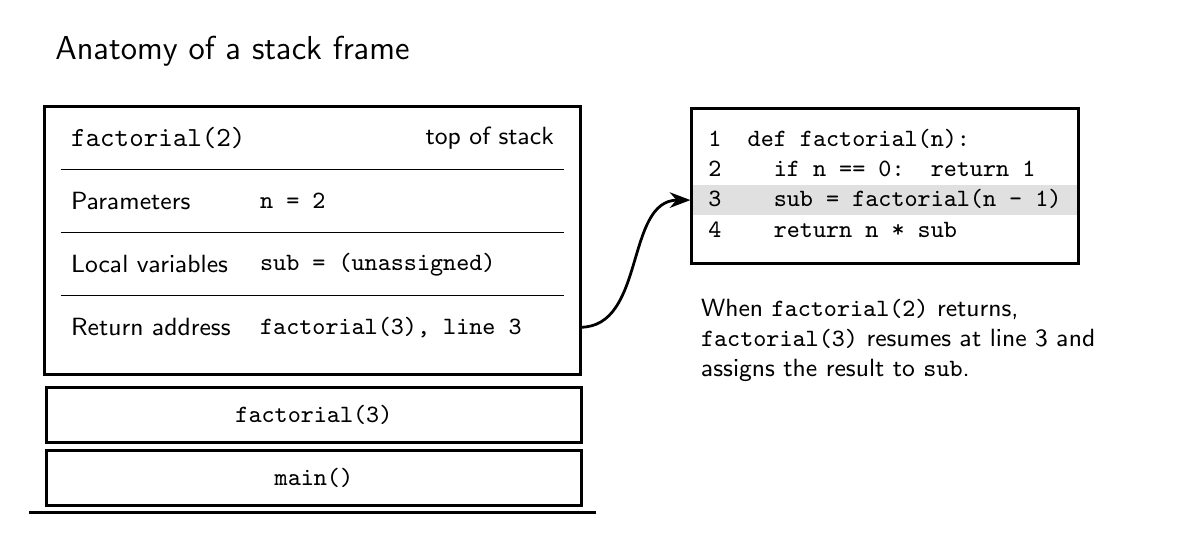
\begin{tikzpicture}[frame/.style={draw, minimum width=6.8cm, minimum height=0.7cm, font=\ttfamily\small},
    code/.style={draw, font=\ttfamily\small, inner sep=6pt}, small/.style={font=\small}]
  \node[anchor=west, font=\large] at (0, 1.1) {Anatomy of a stack frame};
  % The frame on top of the stack, with its three parts.
  \draw (0, 0.4) rectangle (6.8, -3);
  \node[anchor=west, font=\ttfamily] at (0.2, 0) {factorial(2)};
  \node[anchor=east, small] at (6.6, 0) {top of stack};
  \foreach \y/\part/\value in {-0.8/Parameters/{n = 2}, -1.6/Local variables/{sub = (unassigned)},
      -2.4/Return address/{factorial(3), line 3}} {
    \draw[thin] (0.2, \y + 0.4) -- (6.6, \y + 0.4);
    \node[anchor=west, small] at (0.2, \y) {\part};
    \node[anchor=west, font=\ttfamily\small] (v) at (2.6, \y) {\value};
  }
  \coordinate (ret) at (6.8, -2.4);
  \node[frame, anchor=north west] at (0, -3.15) {factorial(3)};
  \node[frame, anchor=north west] at (0, -3.95) {main()};
  \draw (-0.2, -4.75) -- (7, -4.75);

  % The return address points back into the caller's code.
  \node[code, anchor=north west] (code) at (8.2, 0.4) {%
    \begin{tabular}{@{}r@{\quad}l@{}}
      1 & def factorial(n): \\
      2 & \ \ if n == 0: return 1 \\
      3 & \ \ sub = factorial(n - 1) \\
      4 & \ \ return n * sub
    \end{tabular}};
  \fill[black, fill opacity=0.12] ([yshift=-0.99cm]code.north west) rectangle ([yshift=-1.38cm]code.north east);
  \draw[->] (ret) to[out=0, in=180] ([yshift=-1.185cm]code.north west);
  \node[anchor=north west, small, text width=5.6cm] at ([yshift=-0.3cm]code.south west)
    {When \texttt{factorial(2)} returns, \texttt{factorial(3)} resumes at line 3 and assigns the result to \texttt{sub}.};
\end{tikzpicture}
\end{document}
